\documentclass[aspectratio=169,11pt]{beamer}
% Оформление: examples/Эконометрика/Презентация_Дугарев_Хмельницкий_Русских.tex.
% Все результаты: Paper/main.tex; номера таблиц заданы их label в комментариях.
\usepackage{fontspec}
\usepackage{polyglossia}
\setdefaultlanguage{russian}
\setotherlanguage{english}
\setsansfont{Arial}
\newfontfamily\cyrillicfontsf{Arial}
\usepackage{amsmath,amssymb,mathtools,booktabs,array,graphicx,ragged2e,colortbl}
\hyphenpenalty=10000
\usepackage{tikz}
\usetikzlibrary{arrows.meta,positioning}
% Числа для презентации и речи. Источники: Paper/main.tex.
% tab:impacts и пояснение после таблицы.
\newcommand{\CompetitorEffect}{-0{,}027}
\newcommand{\CompetitorPercent}{2{,}66\%}
% tab:sdm, tab:robustness.
\newcommand{\SpatialCoefficient}{0{,}474}
\newcommand{\RegionalSpatialCoefficient}{0{,}204}
% Часть II, Выводы. MAPE восстановлена по округленным баллам.
\newcommand{\InitialScore}{90{,}78}
\newcommand{\FinalScore}{90{,}83}
\newcommand{\InitialMape}{4{,}7215\%}
\newcommand{\FinalMape}{4{,}6952\%}
\newcommand{\MapeGain}{0{,}0262}

\definecolor{main}{HTML}{35444D}
\definecolor{accent}{HTML}{4F8DB7}
\definecolor{pale}{HTML}{EEF4F7}
\definecolor{alertred}{HTML}{9A3A3F}
\definecolor{selectedweight}{HTML}{24764A}
% Part I only: significant estimates / supportive checks, failed diagnostics,
% and partial or borderline evidence. Never infer test success from p alone.
\colorlet{resultgreen}{selectedweight}
\definecolor{resultamber}{HTML}{986000}
\newcommand{\resultok}[1]{\textcolor{resultgreen}{#1}}
\newcommand{\resultbad}[1]{\textcolor{alertred}{#1}}
\newcommand{\resultmixed}[1]{\textcolor{resultamber}{#1}}
\setbeamercolor{normal text}{fg=main,bg=white}
\setbeamercolor{frametitle}{fg=white,bg=main}
\setbeamercolor{title}{fg=white,bg=main}
\setbeamercolor{structure}{fg=accent}
\setbeamercolor{block title}{fg=white,bg=accent}
\setbeamercolor{block body}{fg=main,bg=pale}
\setbeamercolor{alerted text}{fg=alertred}
\setbeamerfont{frametitle}{size=\Large}
\setbeamerfont{block title}{series=\bfseries}
\setbeamertemplate{navigation symbols}{}
\setbeamertemplate{blocks}[rounded][shadow=true]
\setbeamersize{text margin left=7mm,text margin right=7mm}
\setbeamertemplate{frametitle}{%
 \nointerlineskip
 \begin{beamercolorbox}[wd=\paperwidth,ht=0.72cm,dp=0.20cm,leftskip=0.45cm]{frametitle}
 \usebeamerfont{frametitle}\insertframetitle
 \end{beamercolorbox}}
\setbeamercolor{author in head/foot}{bg=main}
\setbeamercolor{title in head/foot}{bg=main}
\setbeamercolor{date in head/foot}{bg=main}
\newcommand{\MainSlideTotal}{25}
\newcommand{\SlideNumber}{\insertframenumber\,/\,\MainSlideTotal}
\newcommand{\FooterFont}{\fontsize{7}{8}\selectfont}
\setbeamertemplate{footline}{%
 \leavevmode\hbox{%
 \begin{beamercolorbox}[wd=.55\paperwidth,ht=2.6ex,dp=1.1ex,leftskip=1.3ex]{author in head/foot}
 \color{white}\FooterFont Гончаров, Дугарев, Русских, Смирнов, Хмельницкий
 \end{beamercolorbox}%
 \begin{beamercolorbox}[wd=.30\paperwidth,ht=2.6ex,dp=1.1ex,center]{title in head/foot}
 \color{white}\FooterFont Пространственная эконометрика
 \end{beamercolorbox}%
 \begin{beamercolorbox}[wd=.15\paperwidth,ht=2.6ex,dp=1.1ex,rightskip=1.3ex plus1fil]{date in head/foot}
 \color{white}\FooterFont 2026 \(\cdot\) \SlideNumber
 \end{beamercolorbox}}}
\newcommand{\good}[1]{\textcolor{accent}{\bfseries #1}}
\newcommand{\tightitems}{\setlength{\itemsep}{0.45em}\setlength{\parskip}{0pt}}
\newcommand{\source}[1]{\par\vspace{1.5mm}{\fontsize{8}{9}\selectfont #1\par}}
\newcommand{\reading}[1]{\par\vspace{3mm}\small\textbf{#1}\par}
\hypersetup{pdftitle={Пространственные эффекты в выручке продуктового ритейла},pdfauthor={Гончаров Алексей, Дугарев Денис, Русских Никита, Смирнов Владимир, Хмельницкий Богдан},pdfsubject={Домашнее задание по пространственной эконометрике}}
% Original Vladimir slides: only theme aliases and typography adaptation.
\newcommand{\VladimirText}{\fontsize{9}{10.5}\selectfont}
\newcommand{\hl}[1]{\good{#1}}
\colorlet{hsedark}{main}
\colorlet{hseblue}{accent}
\colorlet{hselight}{pale}
\colorlet{hsegray}{main!85}
\colorlet{posgreen}{accent}
\begin{document}

% Source: Титульная страница Paper.
\begin{frame}[plain]
\vspace{0.2cm}
\begin{beamercolorbox}[rounded=true,shadow=true,sep=0.4cm,center]{title}
{\large\bfseries Пространственная эконометрика}\par\vspace{0.28cm}
{\LARGE Пространственные эффекты\\в выручке продуктового ритейла}\par\vspace{0.24cm}
{\normalsize Моделирование розничного товарооборота магазинов\\сети «Пятерочка» по локальным рынкам России}
\end{beamercolorbox}
\vspace{0.65cm}\centering
{\normalsize Гончаров Алексей \(\cdot\) Дугарев Денис \(\cdot\) Русских Никита\\[0.15cm]
Смирнов Владимир \(\cdot\) Хмельницкий Богдан}\par
\vspace{0.5cm}{\small Домашнее задание}\par
\vspace{0.4cm}{\small Москва, 2026}
\end{frame}

% Source: Paper, Введение.
\begin{frame}{Вопрос исследования и план}
\begin{block}{Исследовательский вопрос}
Как выручка магазина связана с конкуренцией и окружением соседних локальных рынков?
\end{block}
\vspace{2mm}
\begin{enumerate}\tightitems
\item \textbf{Часть I. Объяснение выручки}\\
\small Данные и гипотезы; срез, панель, динамика и GWR; выводы
\item \normalsize\textbf{Часть II. Прогноз на март 2025 года}\\
\small Ансамбль бустингов; пространственные признаки; качество прогноза
\end{enumerate}
\vspace{3mm}\small Соседство может расширять спрос и одновременно усиливать конкуренцию
\end{frame}


% User-requested section divider; no additional empirical claim.
\begingroup
\setbeamertemplate{frametitle}{}
\begin{frame}[label=part-one]{Часть I. Пространственная эконометрика}
\begin{tikzpicture}[remember picture,overlay]
\node[align=center,text=main] at (current page.center) {\Large Часть I.\\[4mm]\LARGE\bfseries Пространственная эконометрика};
\end{tikzpicture}
\end{frame}
\endgroup

% Source: Paper, Данные, строки 235-381; табл. descriptive.
\begin{frame}{Данные: локальный рынок и выручка магазина}
\small
\textbf{X5 Group + Росстат + GeoNames.} Январь 2023 - февраль 2025\\[1.5mm]
933 населенных пункта, 67 регионов, 15\,683 магазина; не менее 3 магазинов сети на рынок. Панель: $933\times26=24\,258$
\begin{block}{Зависимая переменная: панель и срез}
\vspace{2mm}
\begin{columns}[T,onlytextwidth]
\begin{column}{.58\linewidth}
\small\textbf{Панель: рынок $i$, месяц $t$}
\[
y_{it}=\ln\!\left(\frac1{n_i}\sum_{k\in i}RTO^{\mathrm{real}}_{kt}\right)
\]
\end{column}
\begin{column}{.38\linewidth}
\small\textbf{Срез: среднее за 26 месяцев}
\[
\bar y_i=\frac1{26}\sum_{t=1}^{26}y_{it}
\]
\end{column}
\end{columns}
\small $n_i$ - число магазинов рынка; реальная выручка в ценах января 2023 года\\
$\bar y_i$ используется в SDM и GWR; $y_{it}$ - в панели и динамике
\end{block}
\textbf{Признаки:} население, домохозяйства, пеший и автомобильный трафик; конкуренты и плотность сети; инфраструктура и формат магазина; зарплата и безработица
\source{Координаты доступны на уровне населенного пункта; агрегирование снижает индивидуальный шум. Выводы относятся к рынкам с несколькими магазинами сети}
\end{frame}

% Paper, Данные, fig:location; original Analysis/assets/settlements_russia.png.
% Source: Paper, fig:location; Analysis/assets/settlements_russia.png.
\begin{frame}{Локальные рынки в нашей выборке}
\centering
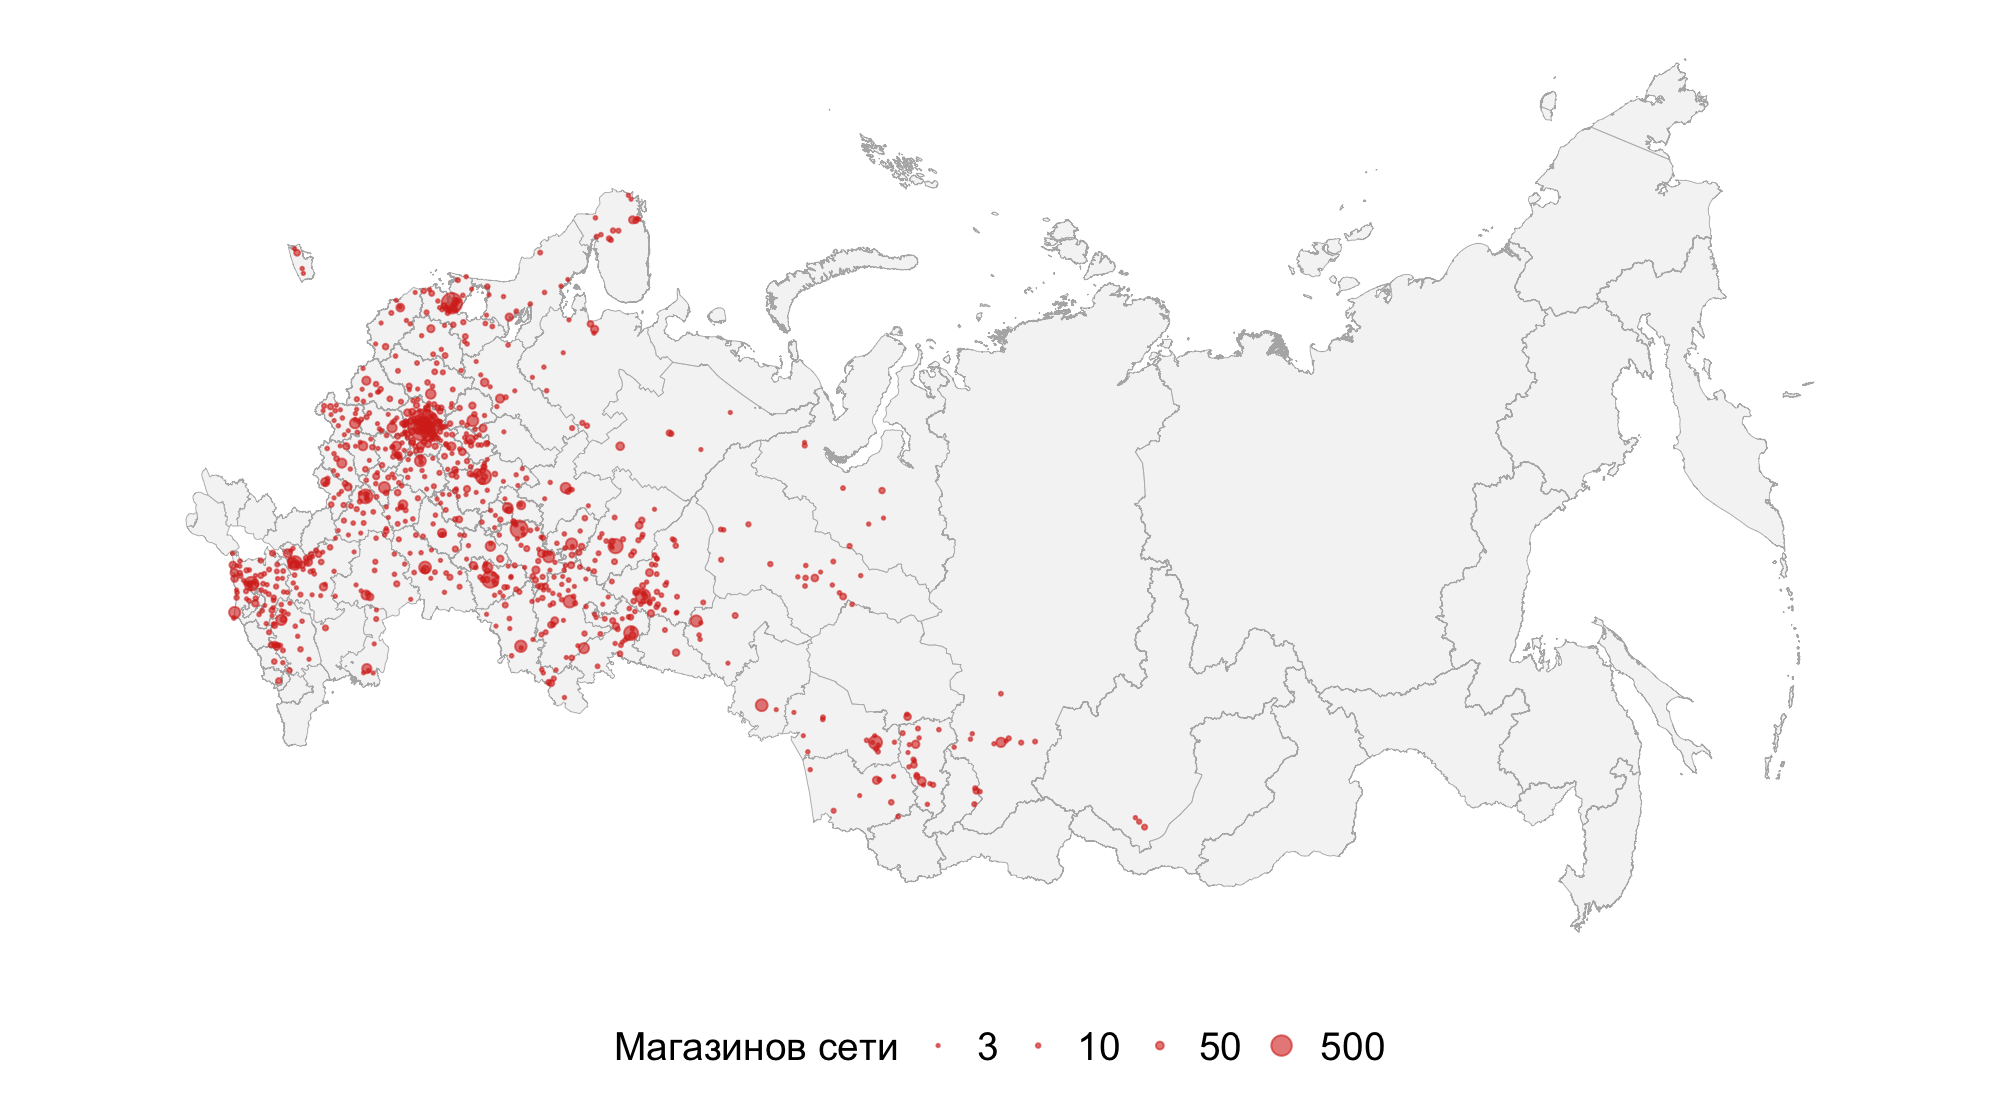
\includegraphics[width=\linewidth,height=.74\textheight,keepaspectratio]{assets/settlements_russia.png}
\source{933 населенных пункта в 67 субъектах. Размер точки - число магазинов сети. Источник: расчеты авторов по X5 Group и GeoNames}
\end{frame}

% Source: Paper, Гипотезы, 697-764.
\begin{frame}{Гипотезы: конкуренция и связи соседних рынков}
\small
\begin{tabular}{@{}p{.07\linewidth}>{\raggedright\arraybackslash}p{.88\linewidth}@{}}
\textbf{H1} & Соседние рынки образуют кластеры схожей выручки\\
& $H_0: I=E(I),\qquad H_1: I>E(I)$\\[1mm]
\textbf{H2} & Связь с выручкой соседей сохраняется при учете характеристик\\
& $H_0:\rho=0,\qquad H_1:\rho\ne0$\\[1mm]
\textbf{H3} & Больше конкурентов и магазинов своей сети - ниже выручка\\
& $H_0:ADE_m=0,\quad H_1:ADE_m<0,\quad m\in\{comp,dens\}$\\[1mm]
\textbf{H4} & Выручка связана с характеристиками соседних рынков\\
& $H_0:AIE_m=0,\qquad H_1:AIE_m\ne0$\\[1mm]
\textbf{H5} & Пространственная модель лучше МНК описывает выручку\\
& $H_0:\rho=0\text{ и }\theta=0,\quad H_1:\rho\ne0\text{ или }\theta\ne0$\\[1mm]
\textbf{H6} & Месячные отклонения соседей связаны после FE рынка и месяца\\
& SAR FE: $H_0:\rho=0,\quad H_1:\rho\ne0$\\
& SEM FE: $H_0:\lambda=0,\quad H_1:\lambda\ne0$
\end{tabular}
\source{ADE/AIE - средние прямой/косвенный эффекты; $comp$ - конкуренты, $dens$ - плотность сети. В H3 и H4 показатели проверяются отдельно}
\end{frame}

% Source: Paper, 450-488, табл. weights, 769-810.
\begin{frame}[label=main-weights]{Матрицы весов: что сравнили и выбрали}
\small
\begin{itemize}\setlength{\itemsep}{0.15em}
\item \textcolor{selectedweight}{\textbf{Экспоненциальные веса: масштаб 50 км, отсечение 300 км}}
\item 8 ближайших соседей (kNN), связи симметризованы
\item Обратные расстояния $1/d$, до 200 км
\item Обратные квадраты расстояний $1/d^2$, до 400 км
\item Пороговая матрица: соседи в радиусе 100 км
\item Экономическая близость: 10 соседей по логарифму населения
\end{itemize}
\[
\widetilde w_{ij}=e^{-d_{ij}/50}\mathbf1\{d_{ij}<300\text{ км}\},\quad
w_{ij}=\frac{\widetilde w_{ij}}{\sum_{k\ne i}\widetilde w_{ik}},\quad w_{ii}=0
\]
\textbf{Почему выбрали:} наибольшее правдоподобие SAR и SDM среди шести W при одинаковых данных и регрессорах
\source{$d_{ij}$ - расстояние в км, 50 км задает скорость убывания весов. Глобальный индекс Морана $\resultok{I=0{,}582}$, $\resultok{p=0{,}001}$ (999 перестановок). Источник: расчеты авторов}
\end{frame}

% Paper, tab:global, fig:moran_scatter, 811-848; original scatter.
% Source: Paper, табл. global, fig:moran_scatter, 811-848.
\begin{frame}{Пространственная связь выручки: глобальные индексы}
\begin{columns}[T,onlytextwidth]
\begin{column}{.64\textwidth}
\centering
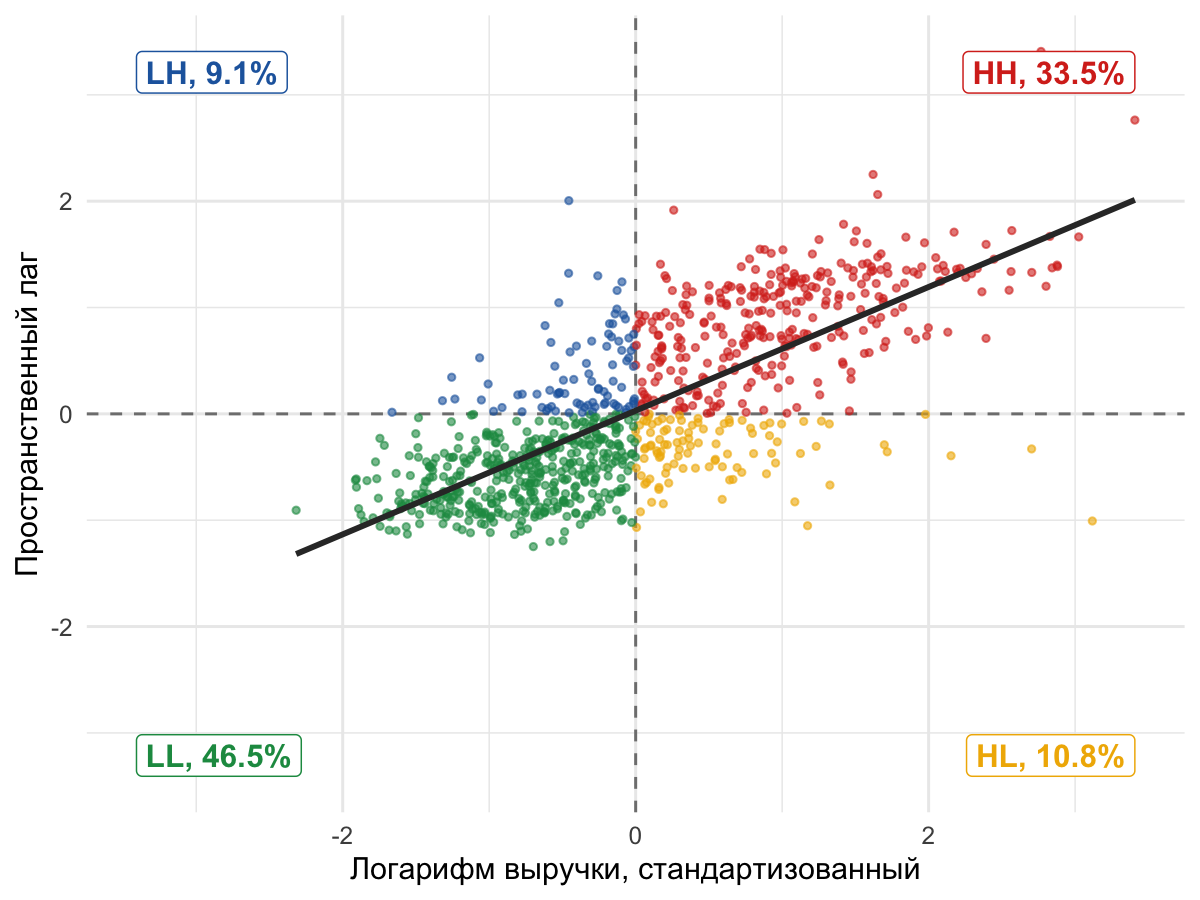
\includegraphics[width=\linewidth,height=.74\textheight,keepaspectratio]{assets/moran_scatter.png}
\end{column}
\begin{column}{.33\textwidth}
\small
\textbf{Глобальный индекс Морана $I$}\\
$\resultok{0{,}582}$, $\resultok{p=0{,}001}$\par\vspace{3mm}
\textbf{Глобальный индекс Гири $C$}\\
$\resultok{0{,}434}$, $\resultok{p<0{,}001}$\par\vspace{3mm}
\textbf{Статистика Гетиса-Орда $G$}\\
$\resultok{0{,}02637}$, $\resultok{p<0{,}001}$\par\vspace{3mm}
\textbf{HH + LL: около 80\% рынков}
\end{column}
\end{columns}
\source{На осях: стандартизованный показатель $\bar y_i$ и его пространственный лаг. Для $I$: 999 перестановок; для $G$: уровни реальной выручки и бинарное соседство 100 км. Источник: расчеты авторов}
\end{frame}

% Paper, fig:local_moran, 857-872. Original asset, not redrawn.
% Source: Paper, fig:local_moran, 857-872.
\begin{frame}{Где находятся кластеры высокой и низкой выручки}
\begin{columns}[T,onlytextwidth]
\begin{column}{.70\textwidth}
\centering
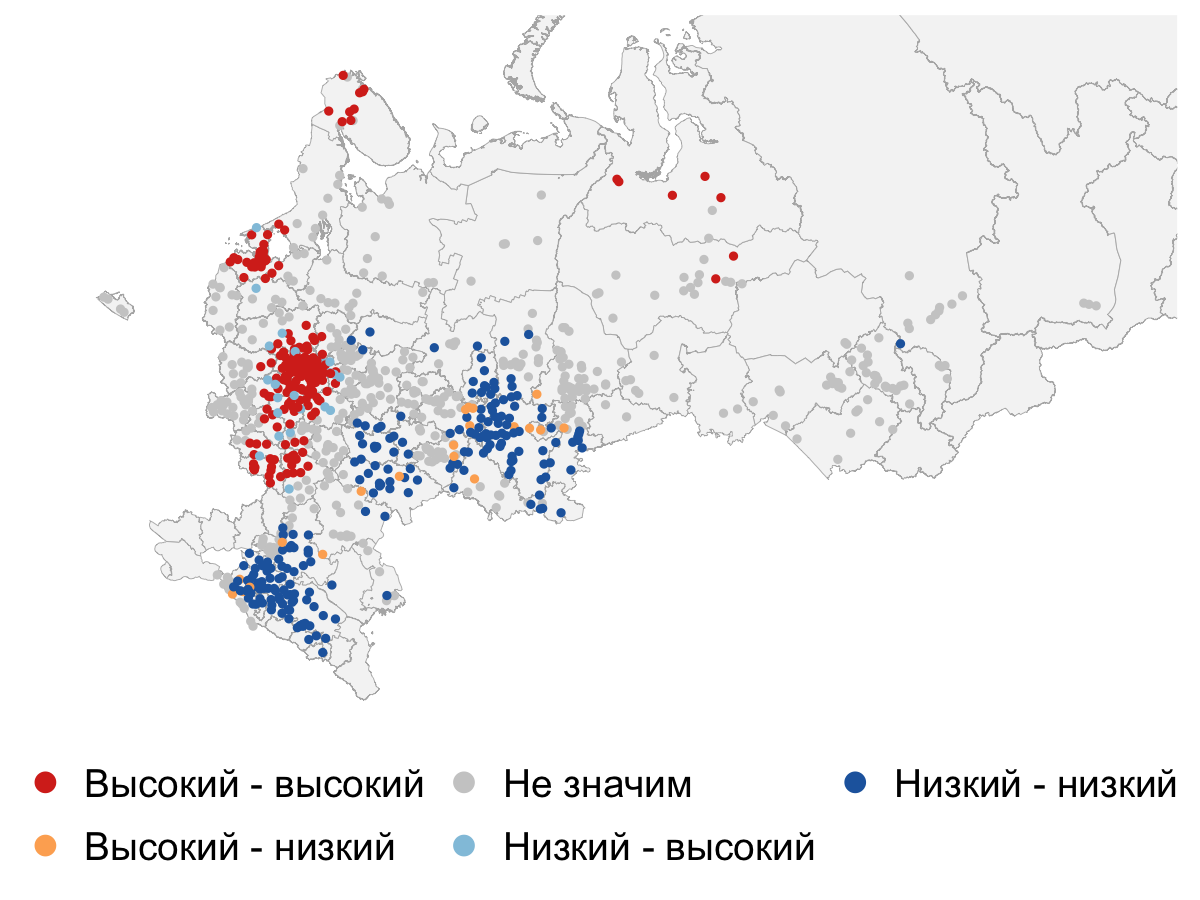
\includegraphics[width=\linewidth,height=.74\textheight,keepaspectratio]{assets/map_local_moran.png}
\end{column}
\begin{column}{.27\textwidth}
\small
\textbf{Локальный индекс Морана $I_i$}\par\vspace{3mm}
\textbf{HH: высокий - высокий}\\
224 населенных пункта\par\vspace{3mm}
\textbf{LL: низкий - низкий}\\
212 населенных пунктов\par\vspace{3mm}
Всего значимы \resultok{\textbf{484 из 933}} рынков
\end{column}
\end{columns}
\source{Границы субъектов сохранены. Двусторонний перестановочный тест, 9999 перестановок, BH-FDR 5\%. Источник: расчеты авторов}
\end{frame}

% Paper, fig:local_getis, fig:local_geary, 874-884; original assets.
% Source: Paper, fig:local_geary, fig:local_getis, 874-884.
\begin{frame}{Локальные статистики: Гири и Гетис-Орд}
\begin{columns}[T,onlytextwidth]
\begin{column}{.49\textwidth}
\centering\small\textbf{Локальный индекс Гири}\par\vspace{1mm}
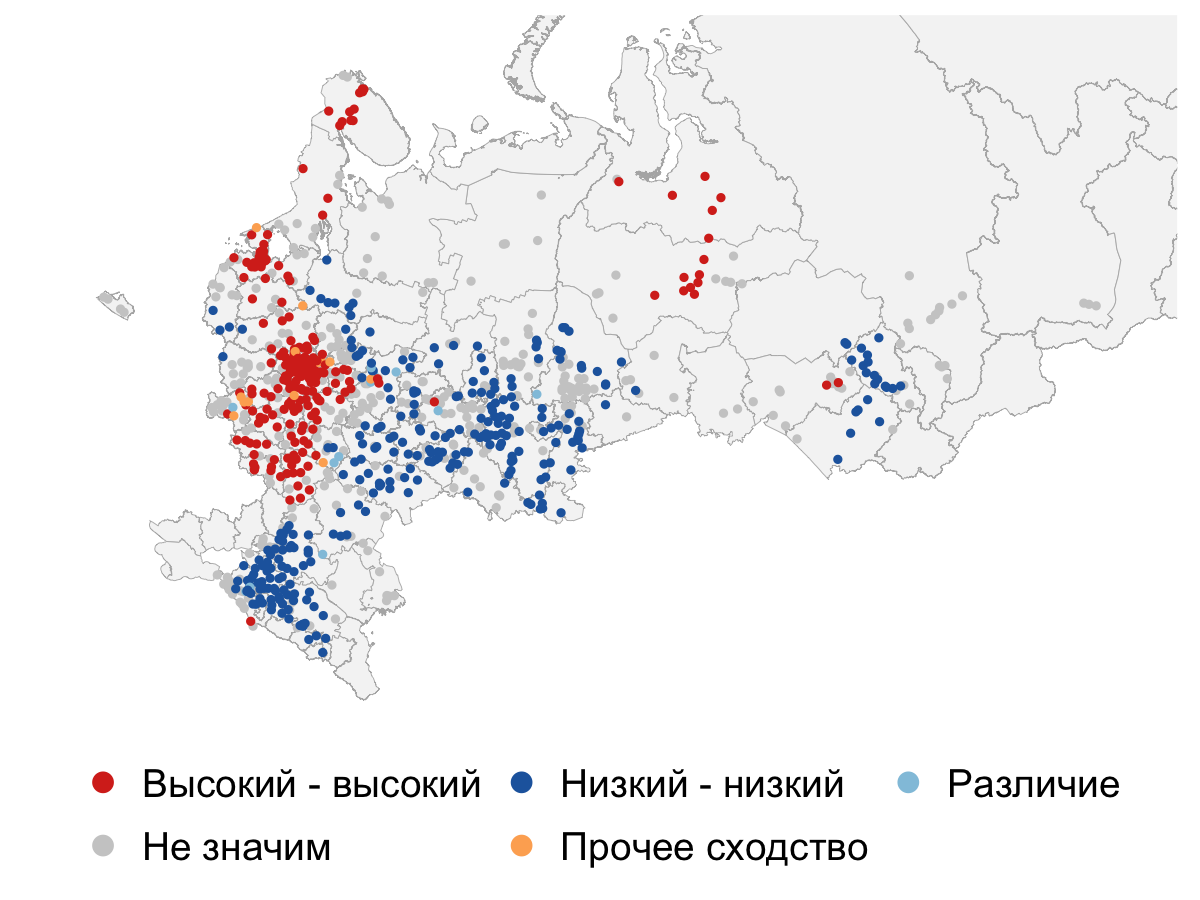
\includegraphics[width=\linewidth,height=.72\textheight,keepaspectratio]{assets/map_local_geary.png}
\end{column}
\begin{column}{.49\textwidth}
\centering\small\textbf{Статистика Гетиса-Орда $G_i^*$}\par\vspace{1mm}
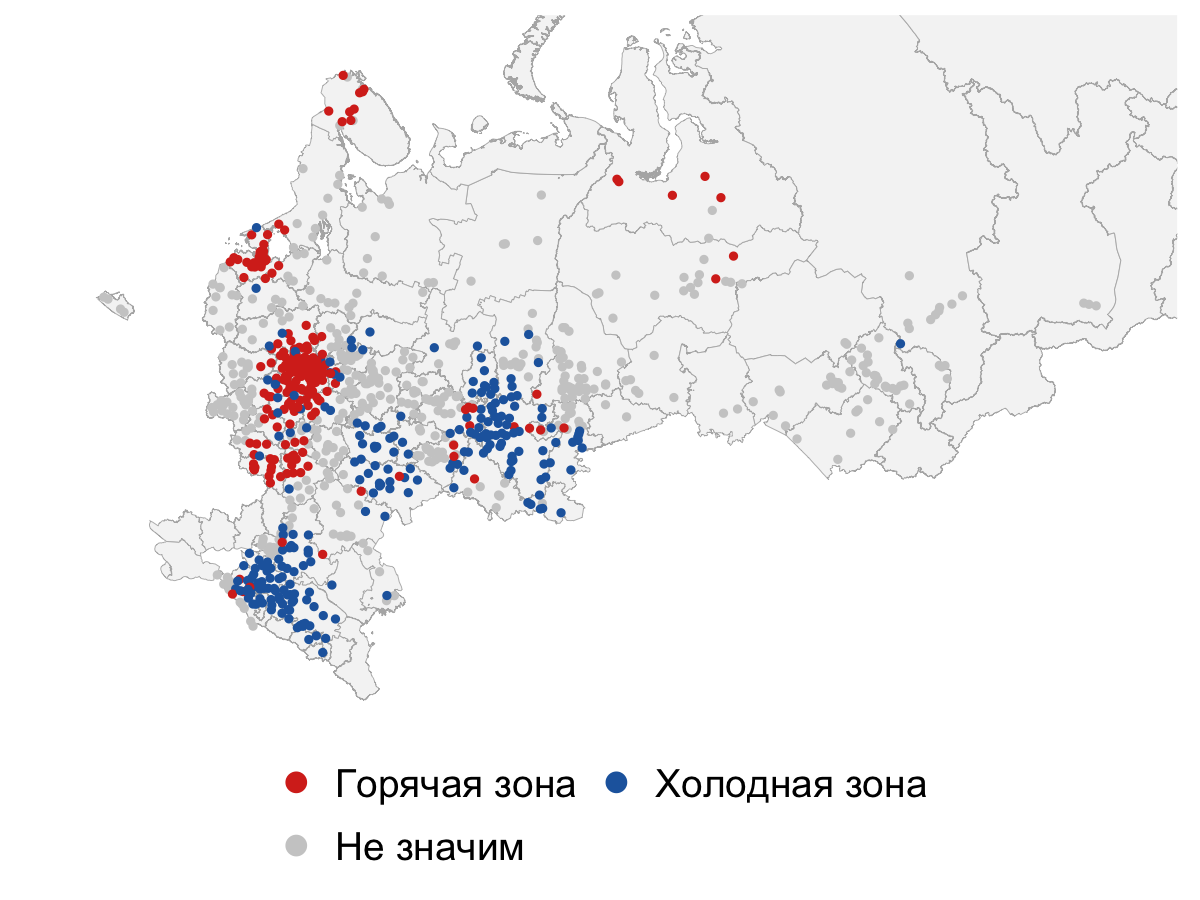
\includegraphics[width=\linewidth,height=.72\textheight,keepaspectratio]{assets/map_local_getis.png}
\end{column}
\end{columns}
\source{BH-FDR 5\%. Гири: \resultok{248} пунктов со сходством высоких и \resultok{294} со сходством низких значений. Гетис-Орд: \resultok{246} пунктов в горячих и \resultok{241} в холодных зонах. Источник: расчеты авторов}
\end{frame}

% Source: Paper, 524-580, 886-965; Source/Seminars, Seminar4.
\begin{frame}[label=main-cross]{Выбор пространственной модели}
\begin{block}{Два подхода к выбору спецификации}
\small
\textbf{От частной к общей:} МНК, LM / робастные LM $\longrightarrow$ SAR\\
\textbf{От общей к частной:} GNS и LR-тесты $\longrightarrow$ SDM
\end{block}
\[
\text{GNS:}\quad \bar y=\rho W\bar y+\alpha\mathbf1+X\beta+WX^{D}\theta+u,\qquad
u=\lambda Wu+\varepsilon
\]
\small
$\rho W\bar y$ - связь усредненной выручки соседей; $X\beta$ - свои характеристики\\
$WX^{D}\theta$ - характеристики соседей; $\lambda Wu$ - зависимость ошибок
\par\vspace{1.5mm}
$X^{D}$: население, домохозяйства, оба вида трафика, конкуренты, плотность сети. В $X$ также входят остальные контроли со слайда данных
\par\vspace{1.5mm}
\textbf{Выбрана SDM:} $\lambda=0$, сохраняются $W\bar y$ и $WX^{D}$
\par LR: $\lambda=0$ в GNS: $\resultok{p=0{,}271}$; $\theta=0$ в SDM: $\resultok{p<0{,}001}$
\source{SAR - предварительный выбор: \resultmixed{оба робастных LM значимы}. Дополнительно: AIC/BIC и остатки; ML и пространственный 2МНК с ошибками Уайта. Инструменты $X,WX,W^2X$ для $W\bar y$ требуют экзогенности $X$}
\end{frame}

% Source: Paper, табл. sdm, impacts, robustness, 1030-1145.
\begin{frame}[label=main-sdm]{SDM: конкуренция и региональная среда}
\small
\centering
\renewcommand{\arraystretch}{1.16}
\begin{tabular}{@{}lrr@{}}
\toprule
 & Основная SDM & SDM + FE субъектов\\
\midrule
$\rho$ & $\resultok{\SpatialCoefficient^{***}}$ & $\resultok{\RegionalSpatialCoefficient^{***}}$\\
Прямой эффект конкурентов & $\resultok{-0{,}027^{***}}$ & $\resultok{-0{,}026^{***}}$\\
Косвенный эффект населения & $\resultok{-0{,}110^{***}}$ & $-0{,}004$\\
Косвенный эффект автотрафика & $\resultok{0{,}121^{**}}$ & $0{,}008$\\
Косвенный эффект плотности сети & $\resultok{0{,}153^{**}}$ & $0{,}075$\\
\bottomrule
\end{tabular}
\source{Источник: расчеты авторов. ML для $\bar y_i$, $N=933$; ** $p<0{,}05$, *** $p<0{,}01$. Для эффектов - 2000 симуляций}
\raggedright
\reading{Связь с конкурентами устойчива; косвенные эффекты зависят от учета регионов}
\small +1 к среднему числу конкурентов в радиусе 500 м: $100(e^{-0{,}027}-1)=\resultok{-2{,}66\%}$. \resultmixed{Прямой эффект собственной сети незначим}
\source{2МНК: $\resultok{\rho=0{,}495}$ (SE $0{,}052$); робастный Wald для $\theta=0$: $\resultok{p<0{,}001}$. AIC предпочитает SDM, BIC - SAR}
\end{frame}

% Source: Paper, 620-639; Analysis/analysis.R, региональная FE-проверка.
\begin{frame}{Панель: связь месячных отклонений}
\small
\[
\begin{aligned}
y_{it}&=\rho\sum_jw_{ij}y_{jt}+x_{it}'\beta+\mu_i+\tau_t+u_{it},\\
u_{it}&=\lambda\sum_jw_{ij}u_{jt}+\varepsilon_{it}
\end{aligned}
\]
\textbf{SARAR FE:} обе компоненты; SAR FE: $\lambda=0$; SEM FE: $\rho=0$
\par\vspace{1.5mm}
$\mu_i$ - постоянный уровень рынка; $\tau_t$ - общий эффект месяца\\
$x_{it}$ - логарифм реальной зарплаты и безработица; постоянные признаки поглощаются $\mu_i$. $N=933$, $T=26$
\begin{block}{Отдельная проверка: эффекты «субъект $\times$ месяц»}
\[
y_{it}=\mu_i+\delta_{r(i),t}+e_{it}
\]
\small $\delta_{r(i),t}$ - свой месячный уровень каждого субъекта
\source{Пространственного лага нет; $W$ используется при проверке остатков. Постоянные признаки поглощены $\mu_i$; зарплата и безработица - $\delta_{r(i),t}$}
\end{block}
\end{frame}

% Source: Paper, табл. panel, 1191-1259.
\begin{frame}[label=main-panel]{Панель: общие шоки имеют значение}
\centering\small
\renewcommand{\arraystretch}{1.1}
\begin{tabular}{@{}lccc@{}}
\toprule
Параметр & SAR FE & SEM FE & SARAR FE\\
\midrule
Лаг выручки $\rho$ & $\resultok{0{,}671^{***}}$ & & $\resultmixed{0{,}357^{*}}$\\
Ошибка $\lambda$ & & $\resultok{0{,}672^{***}}$ & $\resultok{0{,}447^{***}}$\\
\bottomrule
\end{tabular}
\source{ML; * $p<0{,}10$, *** $p<0{,}01$. SARAR: $\resultmixed{p_\rho=0{,}058}$, $\resultok{p_\lambda=0{,}009}$. SE не учитывают связь ошибок во времени}
\source{Средний по месяцам глобальный индекс Морана $I$ остатков: FE $0{,}242$; SAR FE $-0{,}002$; SEM FE $-0{,}001$}
\par\vspace{2mm}
\textbf{Отдельная FE-проверка региональных месячных шоков}\par\vspace{1mm}
\begin{tabular}{@{}>{\raggedright\arraybackslash}m{.46\linewidth}>{\centering\arraybackslash}m{.23\linewidth}>{\centering\arraybackslash}m{.23\linewidth}@{}}
\toprule
Диагностика остатков & FE рынка\newline и месяца & FE рынка и\newline «субъект $\times$ месяц»\\
\midrule
Глобальный индекс Морана $I$\newline Диапазон по месяцам & $0{,}17\ldots0{,}35$ & $-0{,}03\ldots0{,}08$\\
CD-статистика Песарана & $\resultbad{47{,}2^{***}}$ & $\resultbad{26{,}3^{***}}$\\
\bottomrule
\end{tabular}
\raggedright
\reading{Региональные шоки важны; \resultbad{зависимость между рынками сохраняется}}
\end{frame}

% Source: Paper, 641-674.
\begin{frame}{Динамика: инерция и связь во времени}
\small\textbf{Обычная динамическая панель}
\[
y_{it}=\gamma y_{i,t-1}+x_{it}'\beta+\mu_i+\tau_t+\varepsilon_{it}
\]
\small $\gamma$ - инерция выручки. МНК и FE сопоставляются с Ареллано-Бондом и системным GMM; проверяем AR(2) и $J$-тест
\par\vspace{3mm}\textbf{Пространственная динамика}\quad $y_t=(y_{1t},\ldots,y_{Nt})'$
\[
y_t=\gamma y_{t-1}+\rho Wy_t+\eta Wy_{t-1}+X_t\beta+WX_t\theta+\mu+\tau_t\mathbf1+\varepsilon_t
\]
\small $\rho$ - одновременная связь; $\eta$ - связь с прошлой выручкой соседей. В динамической SAR $\theta=0$; в SDM лагируются региональные регрессоры
\begin{block}{Оценивание}
\small ML с двунаправленными FE и коррекцией смещения Ли-Ю. Она нужна из-за смещения порядка $1/T$ при конечном числе месяцев
\end{block}
\end{frame}

% Source: Paper, табл. dynamic, 1263-1327.
\begin{frame}[label=main-dynamic]{Динамика: инерция и ограничения GMM}
\centering\small
\renewcommand{\arraystretch}{1.16}
\begin{tabular}{@{}lccc@{}}
\toprule
Метод & $\widehat\gamma$ (SE) & $J$, $p$ & AR(2), $p$\\
\midrule
МНК с эффектами времени & $0{,}983\;(0{,}002)$ & &\\
FE & $0{,}758\;(0{,}008)$ & &\\
Ареллано-Бонд, лаги 2-4 & $0{,}817\;(0{,}034)$ & $\resultbad{<0{,}001}$ & $\resultok{0{,}226}$\\
Системный GMM, лаги 2-4 & $0{,}958\;(0{,}021)$ & $\resultbad{<0{,}001}$ & $\resultok{0{,}150}$\\
\bottomrule
\end{tabular}
\source{\resultbad{$J$: моментные условия отвергнуты}; \resultok{AR(2): автокорреляция 2-го порядка не выявлена}}
\source{Источник: расчеты авторов. МНК/FE: кластеризация SE по рынкам; GMM: робастные двухшаговые SE. Сопоставимые месяцы 3-26}
\raggedright
\small\vspace{2mm}\textbf{Пространственная SAR после коррекции:} $\resultok{\gamma=0{,}831}$, $\resultok{\rho=0{,}643}$, $\resultok{\eta=-0{,}520}$. Ограничение $\eta+\gamma\rho=0$: $\resultmixed{p=0{,}066}$
\reading{Инерция выражена, но \resultbad{GMM не проходит проверку моментных условий}}
\source{Ограничение не отвергается на 5\%; это не доказывает отсутствие передачи прошлой выручки}
\end{frame}

% Source: Paper, 676-692.
\begin{frame}{GWR: одинаковы ли связи по территории?}
\[
\bar y_i=\beta_0(u_i,v_i)+\sum_m\beta_m(u_i,v_i)x_{im}+\varepsilon_i
\]
\small $\bar y_i$ - показатель среза; $(u_i,v_i)$ - координаты рынка. Коэффициенты оцениваются локально, с большим весом ближайших наблюдений
\par\vspace{3mm}
\begin{itemize}\tightitems
\item Адаптивное гауссовское окно: кросс-валидация выбрала \textbf{61 ближайший населенный пункт}
\item Проверяем постоянство коэффициентов и локальные оценки с поправкой Бонферрони
\item Сравниваем GWR, МНК и SDM по \textbf{одному критерию AICc}
\end{itemize}
\begin{block}{Локальные различия связей}
\small Оцениваем все характеристики рынка. Карта конкурентов показывает, где отрицательная связь с выручкой сильнее
\end{block}
\end{frame}

% Paper, fig:gwr_competitors and GWR results, 1330-1364.
% Source: Paper, fig:gwr_competitors, 1330-1364.
\begin{frame}{GWR: конкуренция почти везде отрицательна}
\begin{columns}[T,onlytextwidth]
\begin{column}{.61\textwidth}
\centering
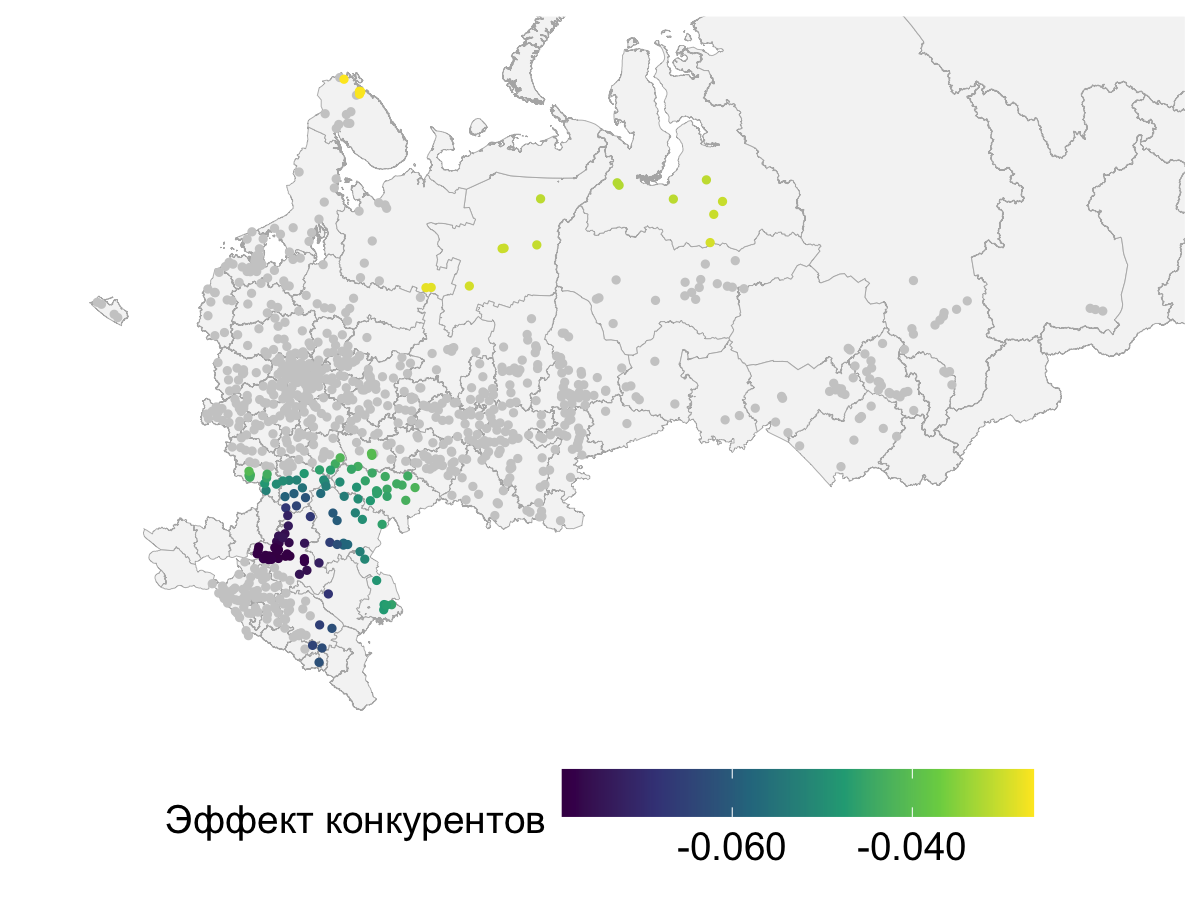
\includegraphics[width=\linewidth,height=.74\textheight,keepaspectratio]{assets/map_gwr_competitors.png}
\end{column}
\begin{column}{.36\textwidth}
\small
\textbf{Локальный коэффициент конкурентов}\\[1mm]
Диапазон: $-0{,}079\ldots0{,}003$\\
Медиана: $-0{,}029$\par\vspace{2mm}
После Бонферрони значимы \resultok{\textbf{124 оценки}}, все отрицательные\par\vspace{2mm}
% Source: Paper/main.tex:1357-1361, significant GWR car-traffic coefficients.
\textbf{Автотрафик:} \resultok{35 значимых оценок}, все положительные\par\vspace{2mm}
\textbf{AICc, меньше лучше}\\[1mm]
\begin{tabular}{@{}lr@{}}
МНК: общие $\beta$ & $-525{,}3$\\
GWR: местные $\beta_i$ & $-730{,}0$\\
SDM: связи соседей & $\resultok{-819{,}6}$
\end{tabular}
\end{column}
\end{columns}
\source{Источник: расчеты авторов. Глобальный индекс Морана $I$ остатков GWR $\resultbad{=0{,}102}$: \resultbad{ошибки пространственно зависимы}, локальная значимость предварительна. Бонферрони структуру ошибок не исправляет}
\end{frame}

% Source: Paper, tab:global (H1), tab:robustness (H2/H4), tab:impacts (H3),
% tab:lr and tab:models (H5), tab:panel and text 1255-1259 (H6).
% H3 density p=0.89 is ML; H6 significance is conditional on ML error assumptions.
\begin{frame}{Часть I: результаты проверки гипотез}
\small
\vspace{2mm}
\renewcommand{\arraystretch}{1.0}
\setlength{\tabcolsep}{4pt}
\begin{tabular}{@{}>{\raggedright\arraybackslash}p{.40\linewidth}>{\raggedright\arraybackslash}p{.56\linewidth}@{}}
\toprule
\textbf{Гипотеза и итог} & \textbf{Показатель из работы}\\
\midrule
\textbf{H1. Кластеры выручки} & Глобальный индекс Морана $\resultok{I=0{,}582}$\\
\resultok{Поддержана} & Перестановочный тест: $\resultok{p=0{,}001}$\\[1mm]
\textbf{H2. Связь выручки соседей} & SDM: $\resultok{\rho=0{,}474^{***}}$\\
\resultok{Поддержана} & С FE субъектов: $\resultok{\rho=0{,}204^{***}}$\\[1mm]
\textbf{H3. Конкуренция и своя сеть} & Конкуренты: $\resultok{ADE=-0{,}027^{***}}$\\
\resultmixed{Частично: только конкуренты} & Плотность сети: $ADE=0{,}002$, $p=0{,}89$\\[1mm]
\textbf{H4. Характеристики соседей} & Население: $\resultok{AIE=-0{,}110^{***}}\to-0{,}004$ с FE\\
\resultmixed{Неустойчива к FE субъектов} & Автотрафик и сеть: с FE незначимы\\[1mm]
\textbf{H5. SDM лучше МНК} & $\resultok{LR=308{,}9}$, $\resultok{p<0{,}001}$\\
\resultok{Поддержана} & AIC: $-525{,}8\to\resultok{-820{,}7}$\\[1mm]
\textbf{H6. Месячная связь соседей} & SAR FE: $\resultok{\rho=0{,}671^{***}}$\\
\resultok{Поддержана при предпосылках ML} & SEM FE: $\resultok{\lambda=0{,}672^{***}}$\\
\bottomrule
\end{tabular}
\source{Условные связи; панельная значимость зависит от предпосылок ML. *** $p<0{,}01$}
\end{frame}


% User-requested section divider; no additional empirical claim.
\begingroup
\setbeamertemplate{frametitle}{}
\begin{frame}[label=part-two]{Часть II. Прогнозирование}
\begin{tikzpicture}[remember picture,overlay]
\node[align=center,text=main] at (current page.center) {\Large Часть II.\\[4mm]\LARGE\bfseries Прогнозирование};
\end{tikzpicture}
\end{frame}
\endgroup

% Full content of Vladimir_part/X5_slides/frames.tex, original frames 1-4.
% Only theme aliases, local 9 pt body, punctuation, subtitle placement and asset path adapted.
% model_scheme.jpg is a byte-identical copy of the explicitly requested original.
\begingroup
\setlength{\abovedisplayskip}{4pt}
\setlength{\belowdisplayskip}{4pt}
\setlength{\abovedisplayshortskip}{3pt}
\setlength{\belowdisplayshortskip}{3pt}
\setlength{\topsep}{2pt}
\setlength{\smallskipamount}{1pt}
\setbeamerfont{block title}{size=\VladimirText}
\setbeamerfont{block body}{size=\VladimirText}
% - 1. Схема исходного решения ------------------------
\begin{frame}[t]{Исходное решение: как устроен ансамбль}
  \VladimirText
  \noindent{Градиентный бустинг для прогноза РТО магазинов за март 2025 года}\par
  
  \begin{columns}[T,onlytextwidth]
    \begin{column}{0.42\textwidth}
      \begin{block}{Подготовка признаков}
        \VladimirText Около \hl{380 признаков}: лаги, скользящие средние, агрегаты и темпы прироста
      \end{block}
      
      \begin{block}{Отбор и настройка}
        \VladimirText Forward Selection: оценка важности на \hl{5 месячных фолдах} с периодическим пересчетом\par
        
        \VladimirText Optuna: взвешенная MAPE на \hl{3 фолдах}
      \end{block}
      
      \begin{block}{Итоговый прогноз}
        \VladimirText Четыре модели с разными признаками и двумя целевыми переменными. Далее - \hl{блендинг}
      \end{block}
    \end{column}
    \begin{column}{0.54\textwidth}
      \centering
      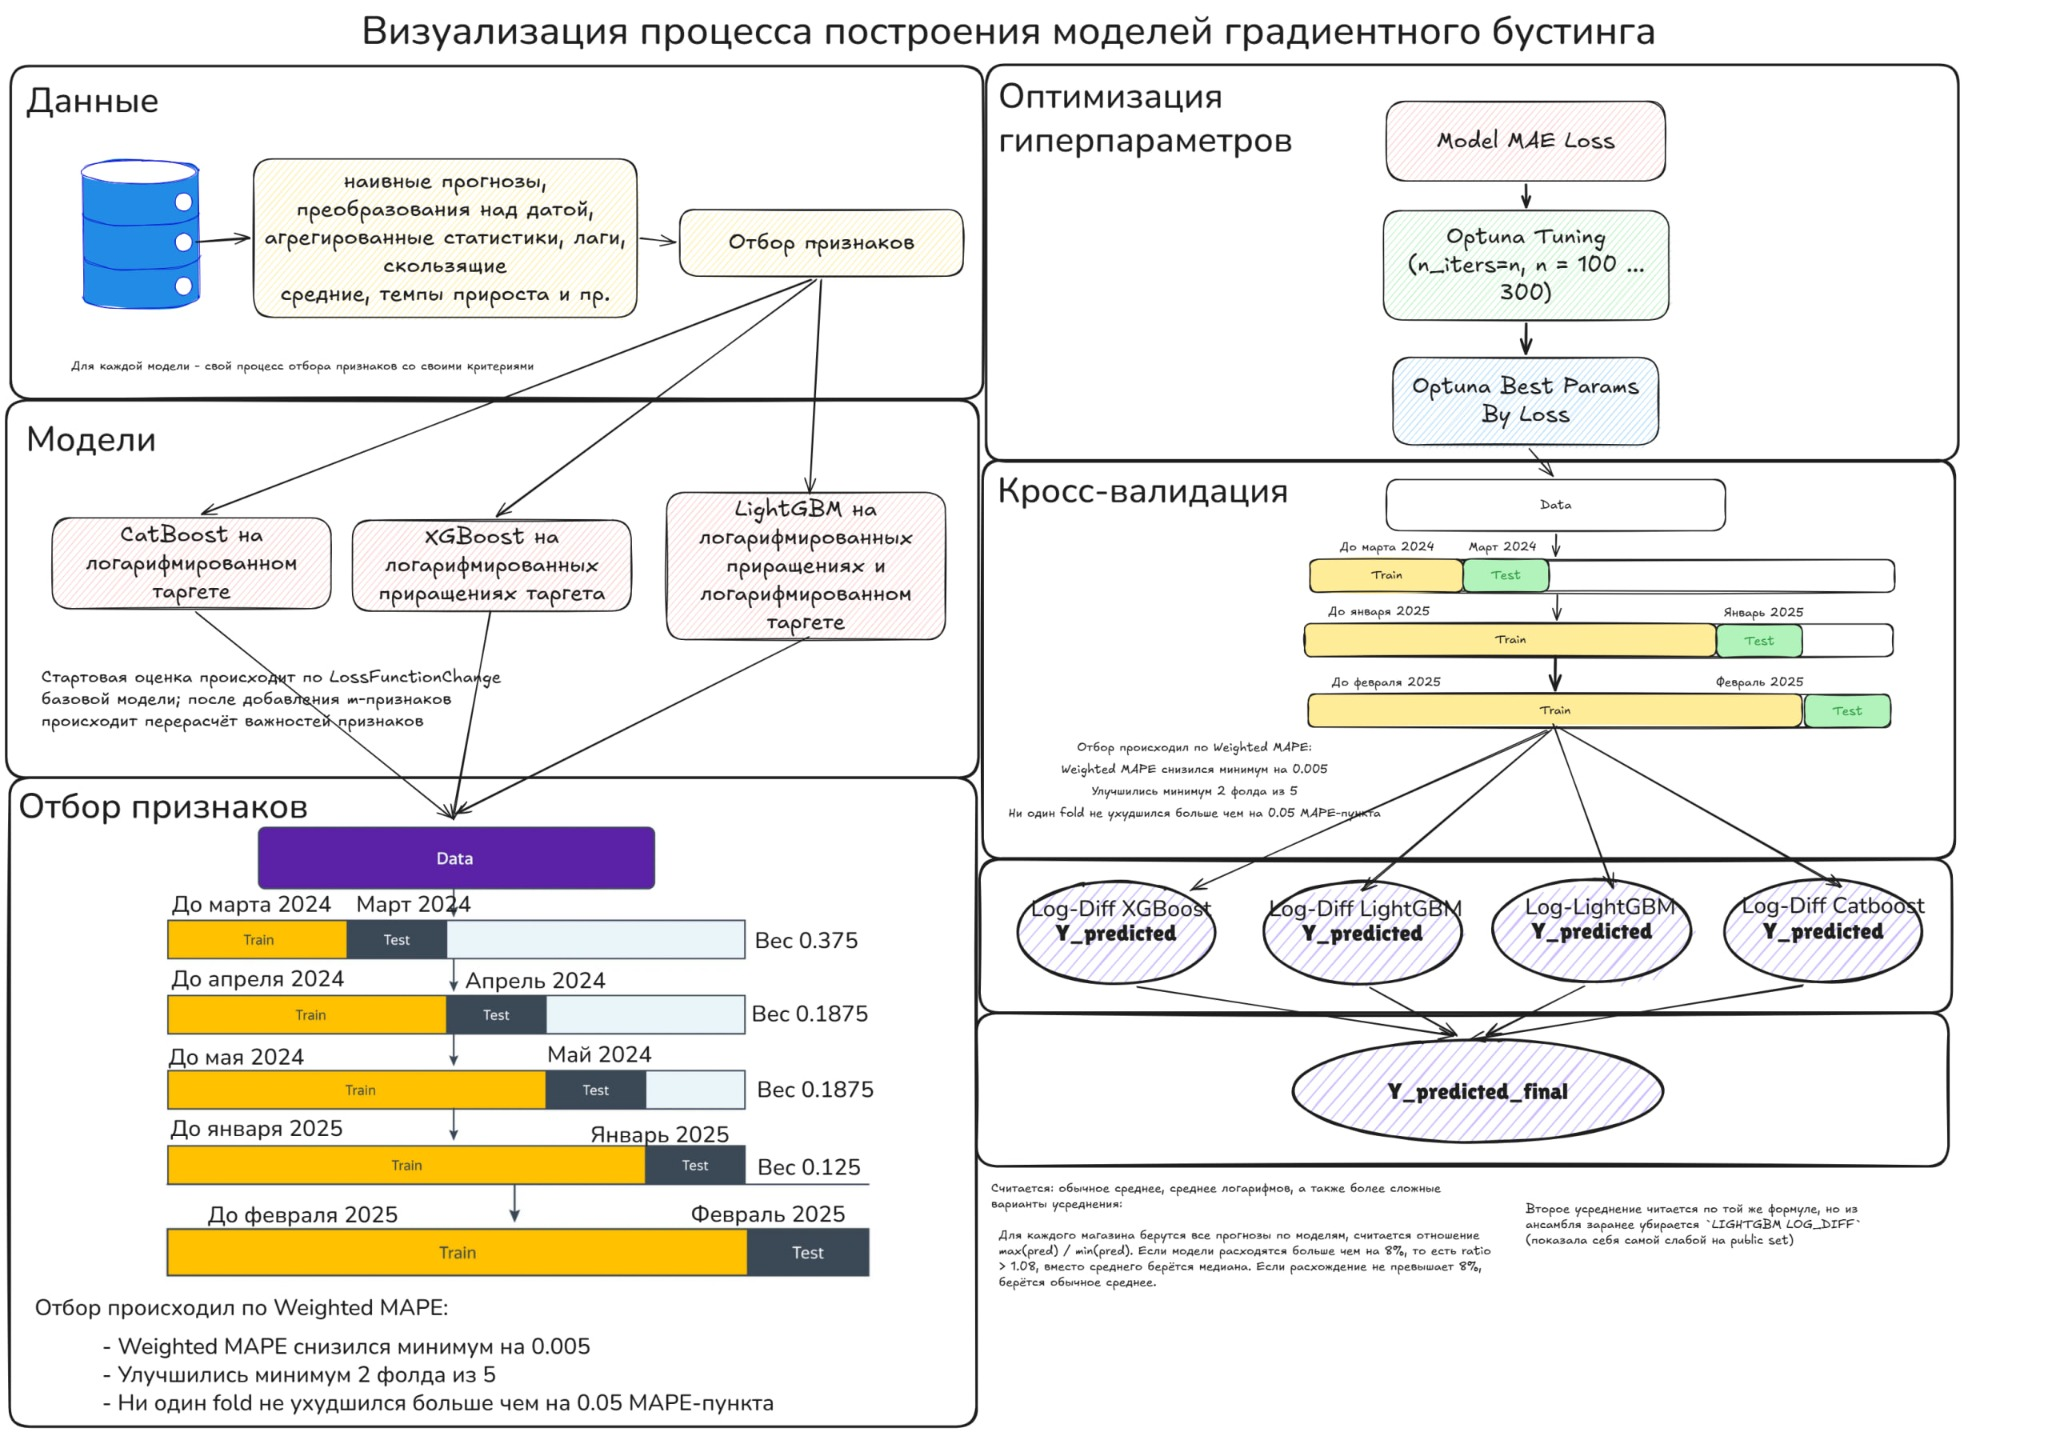
\includegraphics[width=\linewidth,height=.76\textheight,keepaspectratio]{assets/model_scheme.jpg}\par
      
      {\color{hsegray}\fontsize{8}{9}\selectfont Подробная схема обучения, проверки и объединения моделей}
    \end{column}
  \end{columns}
\end{frame}

% - 2. Модели, блендинг и математическая идея -----------------
\begin{frame}[t]{Почему ансамбль может улучшать прогноз?}
  \VladimirText
  \noindent{Разные целевые переменные, наборы признаков и ошибки моделей}\par
  
  \begin{columns}[T,onlytextwidth]
    \begin{column}{0.47\textwidth}
      \begin{block}{Четыре модели в исходном решении}
        \VladimirText
        \setlength{\tabcolsep}{4pt}
        \renewcommand{\arraystretch}{.95}
        \begin{tabular}{@{}ll@{}}
          \toprule
          \textbf{Модель} & \textbf{Целевая переменная} \\
          \midrule
          CatBoost & $\log(1+y)$ \\
          LightGBM уровней & $\log(1+y)$ \\
          LightGBM приростов & $\Delta\log y$ \\
          XGBoost приростов & $\Delta\log y$ \\
          \bottomrule
        \end{tabular}
      \end{block}
      
      {\VladimirText Для каждой модели признаки отбирались отдельно; наборы совпадали лишь частично}\par
      
      \begin{block}{Как объединялись прогнозы}
        \VladimirText Четыре правила: арифметическое, логарифмическое и два пороговых (медиана при расхождении свыше \hl{8\%}). Затем логарифмическое усреднение
      \end{block}
    \end{column}
    \begin{column}{0.49\textwidth}
      \begin{block}{Интуиция снижения дисперсии}
        
        \begin{center}
          {\large\color{hsedark}\(
            E_N=E_1\left(\rho+\frac{1-\rho}{N}\right)
          \)}
        \end{center}
        
        \VladimirText Здесь $N$ - число моделей, $\rho$ - корреляция их ошибок, $E_1$ - дисперсия ошибки одной модели. Формула относится к среднему моделей с одинаковой дисперсией ошибок и общей попарной корреляцией
      \end{block}
      
      \begin{itemize}\VladimirText
        \setlength{\itemsep}{0.8ex}
        \item \hl{Низкая корреляция} ошибок усиливает эффект усреднения
        \item Слишком похожие модели дают небольшой дополнительный выигрыш
        \item Важно сочетать \hl{достаточно точные и разные} прогнозы, а не просто увеличивать число моделей
      \end{itemize}
    \end{column}
  \end{columns}
\end{frame}

% - 3. Пространственные признаки ------------------------
\begin{frame}[t]{Наш эксперимент: пространственные признаки $WX$}
  \VladimirText
  \noindent{Учитываем характеристики соседних населенных пунктов, не меняя исходные модели}\par
  
  \begin{columns}[T,onlytextwidth]
    \begin{column}{0.52\textwidth}
      \begin{block}{От пространственной модели SLX к бустингу}
        \begin{center}
          {\small\color{hsedark}\(y=X\beta+WX\theta+\varepsilon\)}
        \end{center}
        \VladimirText В бустинге $WX$ используется как \hl{дополнительный набор признаков}, без оценивания причинных эффектов SLX
      \end{block}
      
      \begin{enumerate}\VladimirText
        \setlength{\itemsep}{0.65ex}
        \item Строим матрицу весов $W$ по \hl{6 или 12 ближайшим} населенным пунктам, нормируем строки
        \item Усредняем признаки магазинов в каждом пункте и рассчитываем среднее по соседям:
        \[
          (WX)_{rjt}=\sum_v w_{rv}\,\overline{x}_{vjt}
        \]
        \item Присоединяем полученные признаки к наблюдениям магазинов
      \end{enumerate}
    \end{column}
    \begin{column}{0.44\textwidth}
      \begin{block}{Масштаб данных}
        \begin{center}
          \begin{tabular}{@{}cc@{}}
            {\Large\bfseries\color{hseblue}18\,657} & {\Large\bfseries\color{hseblue}3\,360} \\
            {\VladimirText магазинов} & {\VladimirText населенных пунктов}
          \end{tabular}
        \end{center}
      \end{block}
      
      \begin{block}{Количество добавленных $WX$-признаков}
        \VladimirText
        \renewcommand{\arraystretch}{1.35}
        \setlength{\tabcolsep}{2pt}
        \begin{tabular*}{\linewidth}{@{\extracolsep{\fill}}lr@{}}
          CatBoost & \hl{39} \\
          LightGBM приростов & \hl{22} \\
          LightGBM уровней & \hl{33} \\
          XGBoost & \hl{14}
        \end{tabular*}
      \end{block}
      \vspace{0.25ex}
      {\VladimirText\color{hsegray}Для мартовского прогноза использовались только сведения, доступные к концу февраля}
    \end{column}
  \end{columns}
\end{frame}

% - 4. Результаты и ограничения ------------------------
\begin{frame}[t]{Итог: пространственные признаки и качество прогноза}
  \VladimirText
  \noindent{Полный мартовский тест соревнования, балл по MAPE}\par
  
  \begin{columns}[T,onlytextwidth]
    \begin{column}{0.51\textwidth}
      \begin{block}{Результат отдельных составов ансамбля}
        \VladimirText
        \setlength{\tabcolsep}{4pt}
        \renewcommand{\arraystretch}{1.15}
        \begin{tabular*}{\linewidth}{@{\extracolsep{\fill}}lr@{}}
          \toprule
          \textbf{Модели с $WX$} & \textbf{Балл} \\
          \midrule
          Без $WX$ (исходный ансамбль) & 90,78 \\
          Только XGBoost & 90,80 \\
          XGBoost и LightGBM приростов & 90,82 \\
          \rowcolor{hselight}
          \textbf{XGBoost и оба LightGBM} & \textbf{\color{posgreen}90,83} \\
          \bottomrule
        \end{tabular*}
      \end{block}
      
      \begin{itemize}\VladimirText
        \setlength{\itemsep}{0.55ex}
        \item CatBoost в лучшем составе остался \hl{исходным}
        \item XGBoost отдельно: \hl{90,45 $\rightarrow$ 90,58}; оба LightGBM по отдельности ухудшились
        \item Дополнительное усреднение готовых ансамблей не повысило округленный балл
      \end{itemize}
    \end{column}
    \begin{column}{0.45\textwidth}
      \begin{block}{Изменение итоговой метрики}
        \centering
        {\Large\color{hsegray}90,78}
        {\Large\color{hseblue}$\;\longrightarrow\;$}
        {\LARGE\bfseries\color{posgreen}90,83}\par
        
        {\VladimirText MAPE: $4{,}7215\%\;\rightarrow\;4{,}6952\%$}\par
        \vspace{0.25ex}
        {\VladimirText Снижение примерно на \hl{0,0262 процентного пункта}}
      \end{block}
      \vspace{0.25ex}
      \begin{block}{Если пересчитать места в рейтинге}
        \VladimirText Общее место: \hl{21-22 $\rightarrow$ 12}\par
        \vspace{0.45ex}
        \VladimirText Среди приглашенных на защиту: \hl{8 $\rightarrow$ 5}
      \end{block}
      \vspace{0.45ex}
      {\fontsize{8}{9}\selectfont\color{hsegray}\textbf{Ограничение:} составы сравнивались с учетом баллов полного теста. Это не независимая оценка качества на будущих месяцах}
    \end{column}
  \end{columns}
\end{frame}

\endgroup


% User-requested exact repeat of the opening title.
\begin{frame}[plain]
\vspace{0.2cm}
\begin{beamercolorbox}[rounded=true,shadow=true,sep=0.4cm,center]{title}
{\large\bfseries Пространственная эконометрика}\par\vspace{0.28cm}
{\LARGE Пространственные эффекты\\в выручке продуктового ритейла}\par\vspace{0.24cm}
{\normalsize Моделирование розничного товарооборота магазинов\\сети «Пятерочка» по локальным рынкам России}
\end{beamercolorbox}
\vspace{0.65cm}\centering
{\normalsize Гончаров Алексей \(\cdot\) Дугарев Денис \(\cdot\) Русских Никита\\[0.15cm]
Смирнов Владимир \(\cdot\) Хмельницкий Богдан}\par
\vspace{0.5cm}{\small Домашнее задание}\par
\vspace{0.4cm}{\small Москва, 2026}
\end{frame}
\end{document}
